% Tags: 4321102, shift, serial-out, working, serial-in, register
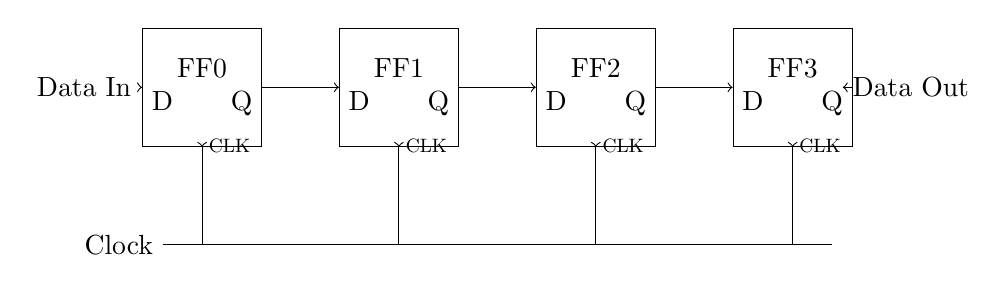
\begin{tikzpicture}[
    node distance=2cm,
    auto,
    block/.style={rectangle, draw, minimum width=1.5cm, minimum height=1.5cm, align=center}
]
    \foreach \i in {0,1,2,3} {
        \node[block] (FF\i) at (\i*2.5, 0) {FF\i\\D \hspace{0.5cm} Q};
        \draw[->] (\i*2.5, -1) -- (\i*2.5, -0.75) node[right, scale=0.7] {CLK} -- (FF\i.south);
    }
    
    \node (Din) at (-1.5, 0) {Data In};
    \draw[->] (Din) -- (FF0.west);
    
    \draw[->] (FF0.east) -- (FF1.west);
    \draw[->] (FF1.east) -- (FF2.west);
    \draw[->] (FF2.east) -- (FF3.west);
    
    \node (Dout) at (9, 0) {Data Out};
    \draw[->] (FF3.east) -- (Dout);
    
    % Clock Line
    \draw (-0.5, -2) node[left] {Clock} -- (8, -2);
    \foreach \i in {0,1,2,3} {
        \draw (\i*2.5, -2) -- (\i*2.5, -1);
    }

\end{tikzpicture}
